%   preamble {{{1  %
%%%%%%%%%%%%%%%%%%%%

\documentclass[handout]{beamer}

\usepackage[utf8]{inputenc}
\usepackage[english]{babel}

%  beamer theme {{{1  %
%%%%%%%%%%%%%%%%%%%%%%%

\usetheme{metropolis}           % Use metropolis theme
\metroset{background=light}
\setbeamertemplate{frame footer}{

\includegraphics[width=1cm, keepaspectratio]{images/max_planck.png}
} %Metropolis defined
\setbeamercolor{background canvas}{bg=white}



\title{
  
\includegraphics[width=2cm, keepaspectratio]{images/max_planck.png}
 \hfill
  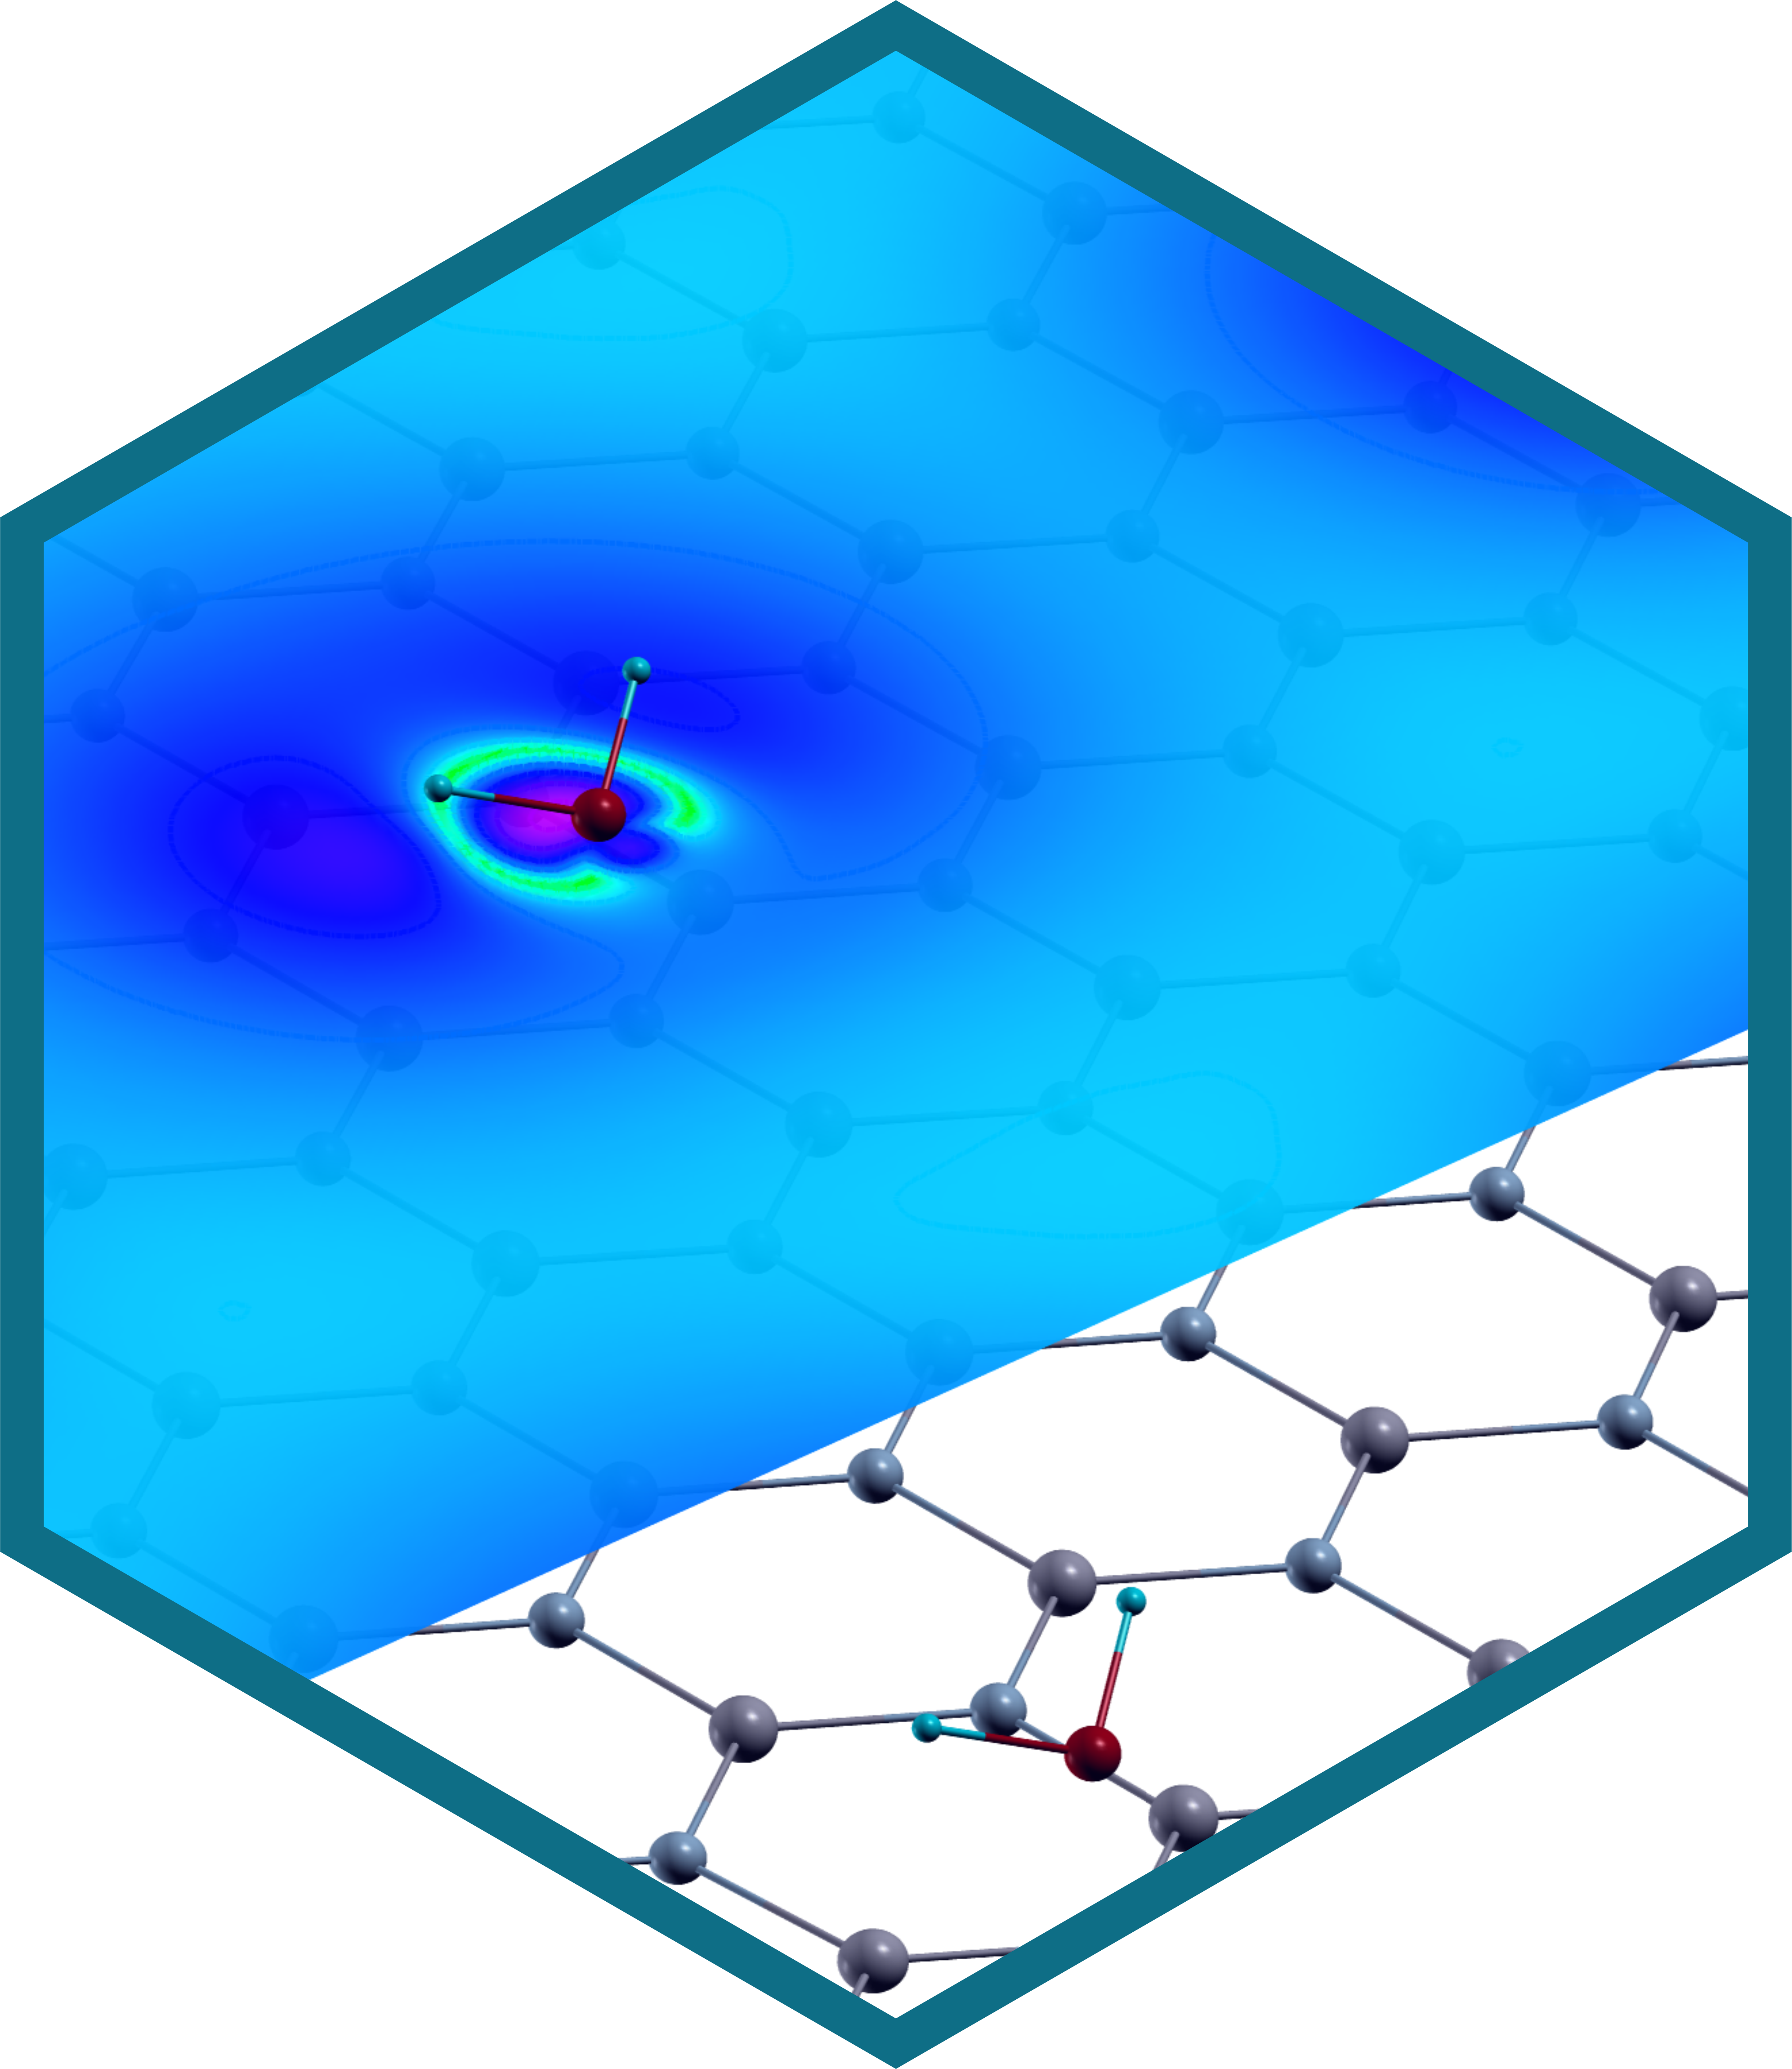
\includegraphics[width=1.4cm, keepaspectratio]{images/logo_andreas.png} \\
  Ab initio studies of vacancy-impurity complexes in cubic and hexagonal
  diamond
}
\date{July 28, 2016}


\author{Alejandro Agustí Martínez-Soria Gallo}
\institute{Max-Planck Institute for solid state research}



\begin{document}


%  title {{{1  %
%%%%%%%%%%%%%%%%

\maketitle


\begin{frame}{Contents}
\tableofcontents
\end{frame}



\section{Aim and scope of the work} %{{{1
\begin{frame}{Aims}
\begin{itemize}
  \item<1->
Exploration of defect centres using state-of-the-art ab-initio theories.
  \item<2->
Reproduce and obtain classical results for nitrogen vacancy impurity complexes in diamond.
  %\item<3->
%What is the state of the art of ab-initio theories?
  %\item<4->
%How can ab-initio methods help in understanding and improving their
%properties?
\end{itemize}
\end{frame}

\section{Introduction} %{{{1


\begin{frame}{Nitrogen Vacancy Centre in diamond}
  \begin{center}
    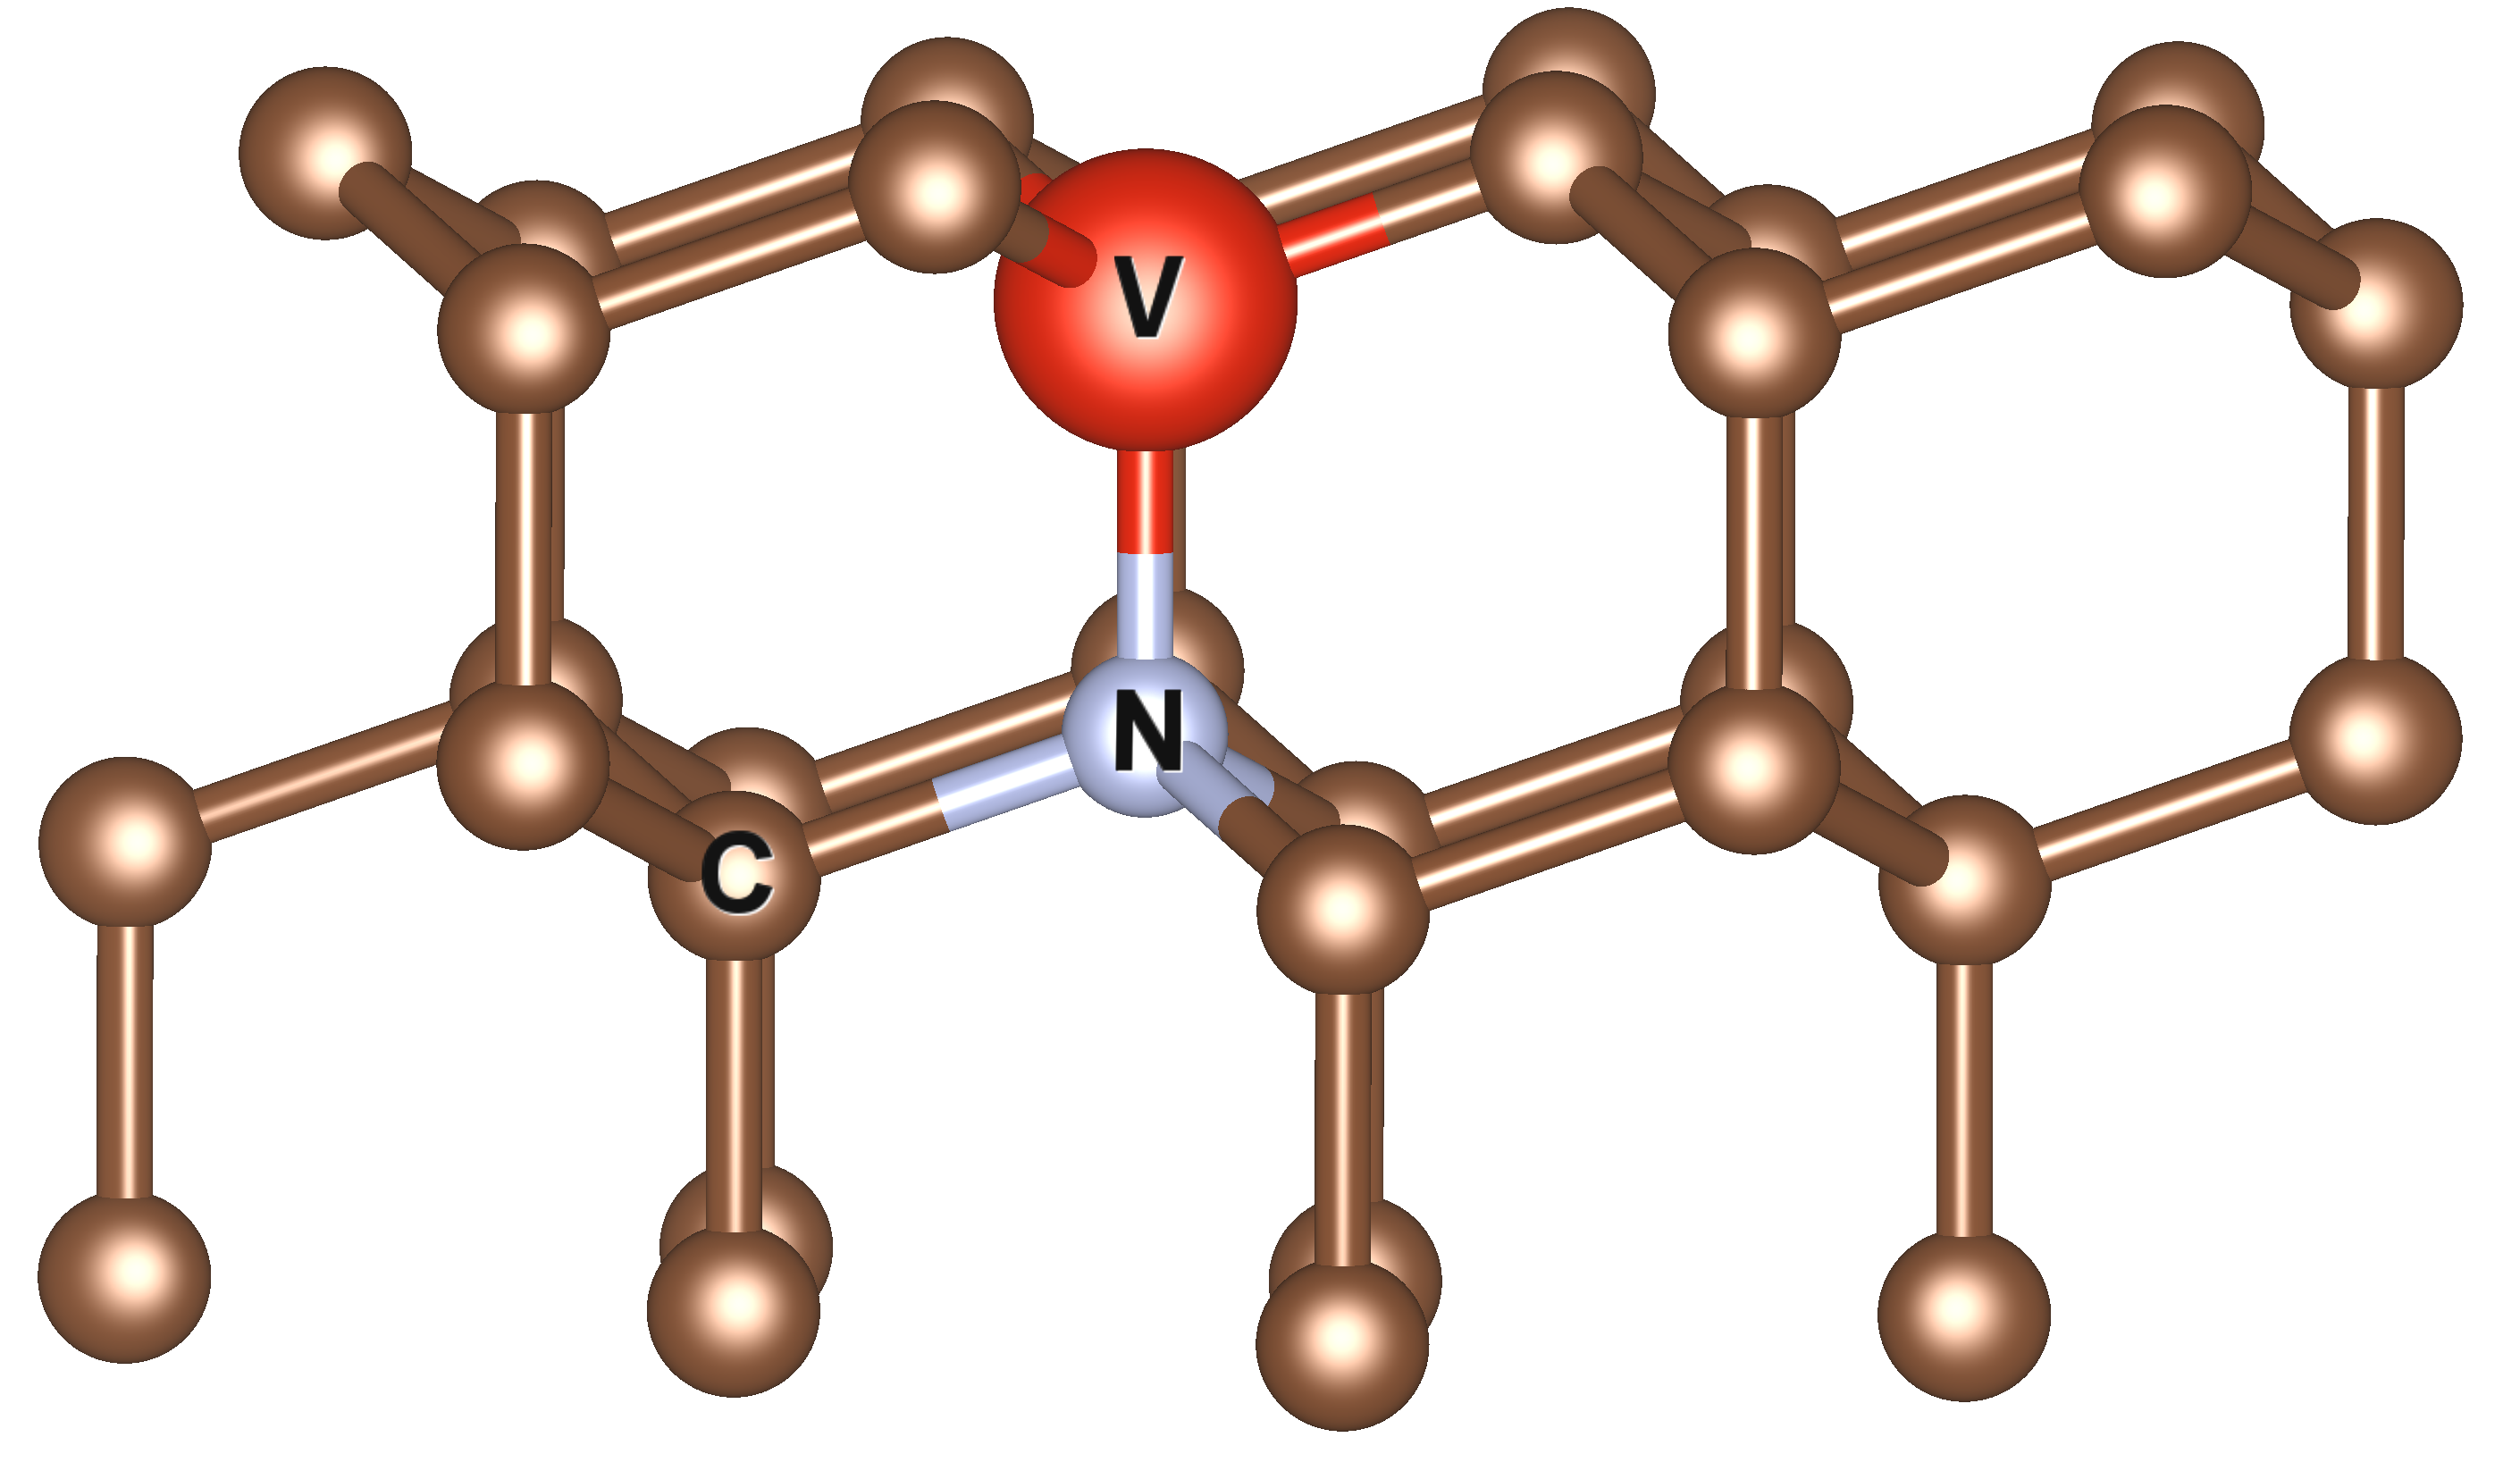
\includegraphics[width=0.9\textwidth]{images/POSCAR_16_view.png}
  \end{center}
\end{frame}

\begin{frame}{Main level overview: $ \mathsf{NV}^{-} $ }
  \begin{center}
    \includegraphics[width=0.7\textwidth]{images/basic_levels.pdf}
  \end{center}
\end{frame}

\begin{frame}{Triplets overview: $ \mathsf{NV}^{-} $ }
  \begin{center}
    \begin{columns}
      \begin{column}{0.5\textwidth}
        \centering
        \includegraphics[height=.8\textheight]{images/basic_levels_triplets.pdf}
      \end{column}
      \begin{column}{0.5\textwidth}
        \centering
        \includegraphics[height=1\textheight]{images/basic_triplet_configuration.pdf}
      \end{column}
    \end{columns}
  \end{center}
\end{frame}

\begin{frame}{Transitions}
  \begin{center}
    \includegraphics[width=0.5\textwidth]{images/splitting.pdf}
  \end{center}
\end{frame}

\begin{frame}{Transitions overview: $ \mathsf{NV}^{-} $ }
  \begin{center}
    \includegraphics[width=0.7\textwidth]{images/NV_minus_transitions.pdf}
  \end{center}
\end{frame}


\begin{frame}{Zero phonon line (ZPL)}
  \begin{columns}
    \begin{column}{0.5\textwidth}
    \includegraphics[width=0.8\textwidth]{images/basic_levels_triplets.pdf}
    \end{column}
    \begin{column}{0.5\textwidth}
    \includegraphics[width=1\textwidth]{images/vibronic.pdf}
    \end{column}
  \end{columns}
\end{frame}

\begin{frame}{Density functional theory (DFT)}
  \textit{``$ \it \Psi  $  contains too much information''}
  \hfill \textit{- Popular saying}
  \begin{itemize}
    \item The exact electronic ground state of a system is only dependent on
      the electronic density $ \rho $ .
    \item In principle, DFT delivers the \textbf{exact ground state}.
    \item All quantities written in terms of $ \rho $ (functional formalism).
    \item E.g.:
      \[
        E[ \rho ] =
        T_{s} [ \rho  ]
        +
        \int  V ( \mathbf{r} ) \rho ( \mathbf{r} ) \ \mathrm{d} \mathbf{r}
        +
        \frac{1}{4\pi \epsilon _{0}}
        \int
        \frac{\rho ( \mathbf{r} ) \rho ( \mathbf{r}' )}{| \mathbf{r} - \mathbf{r}'|}
        \ \mathrm{d} \mathbf{r}\mathrm{d} \mathbf{r}'
        +
        E^{ \mathrm{exact}}_{ \mathrm{xc}} [ \rho ]
      \]
      The exchange correlation potential
      $ E^{ \mathrm{exact}}_{ \mathrm{xc}} [ \rho ] $
      determines the DFT \textit{flavor}.
  \end{itemize}
\end{frame}


%\begin{frame}{Projector-augmented wave (PAW) method}
%\end{frame}


\section{Hexagonal diamond and defects} %{{{1


\begin{frame}{Hexagonal diamond}
  \begin{center}
    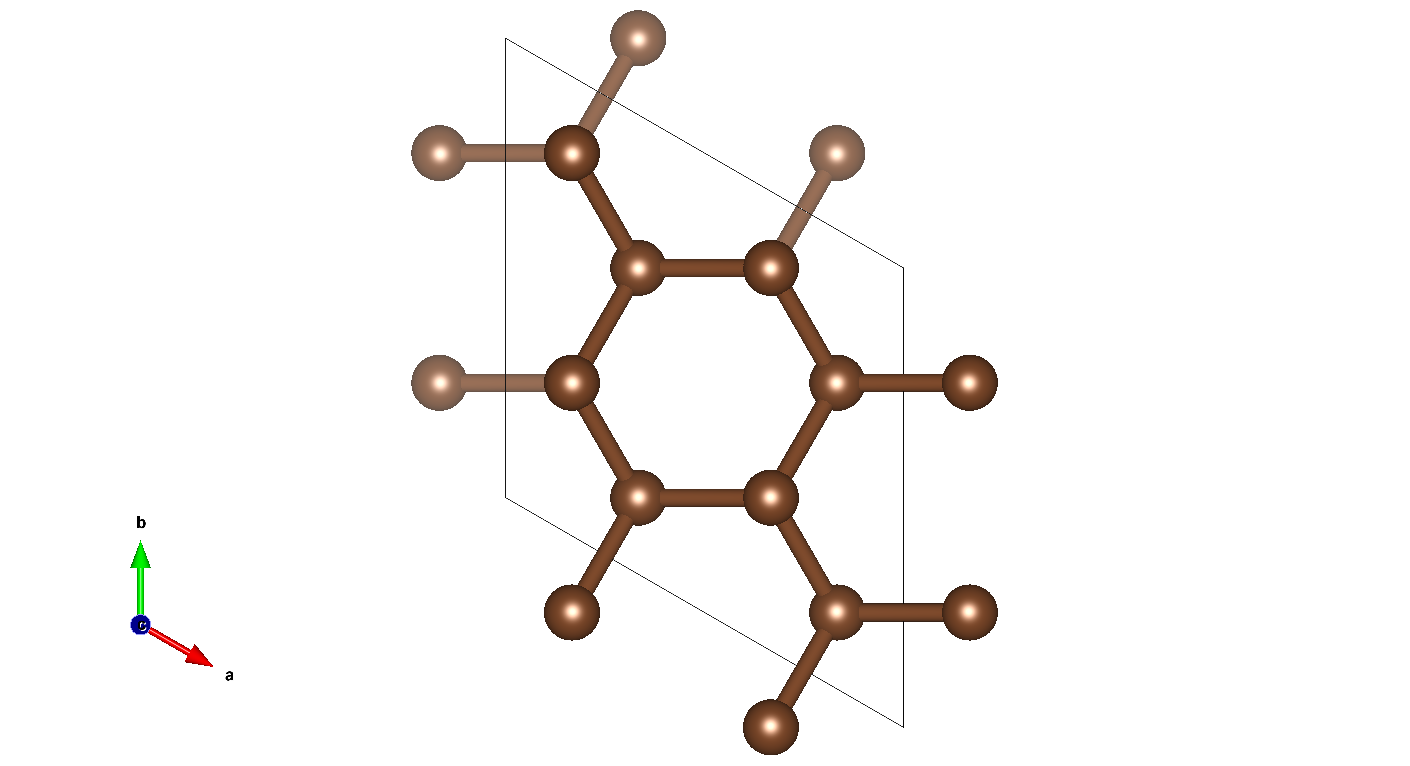
\includegraphics[width=0.5\textwidth, trim=0 0 30em 0,clip]{images/poscar_hex_16_hex-view.png}\\
    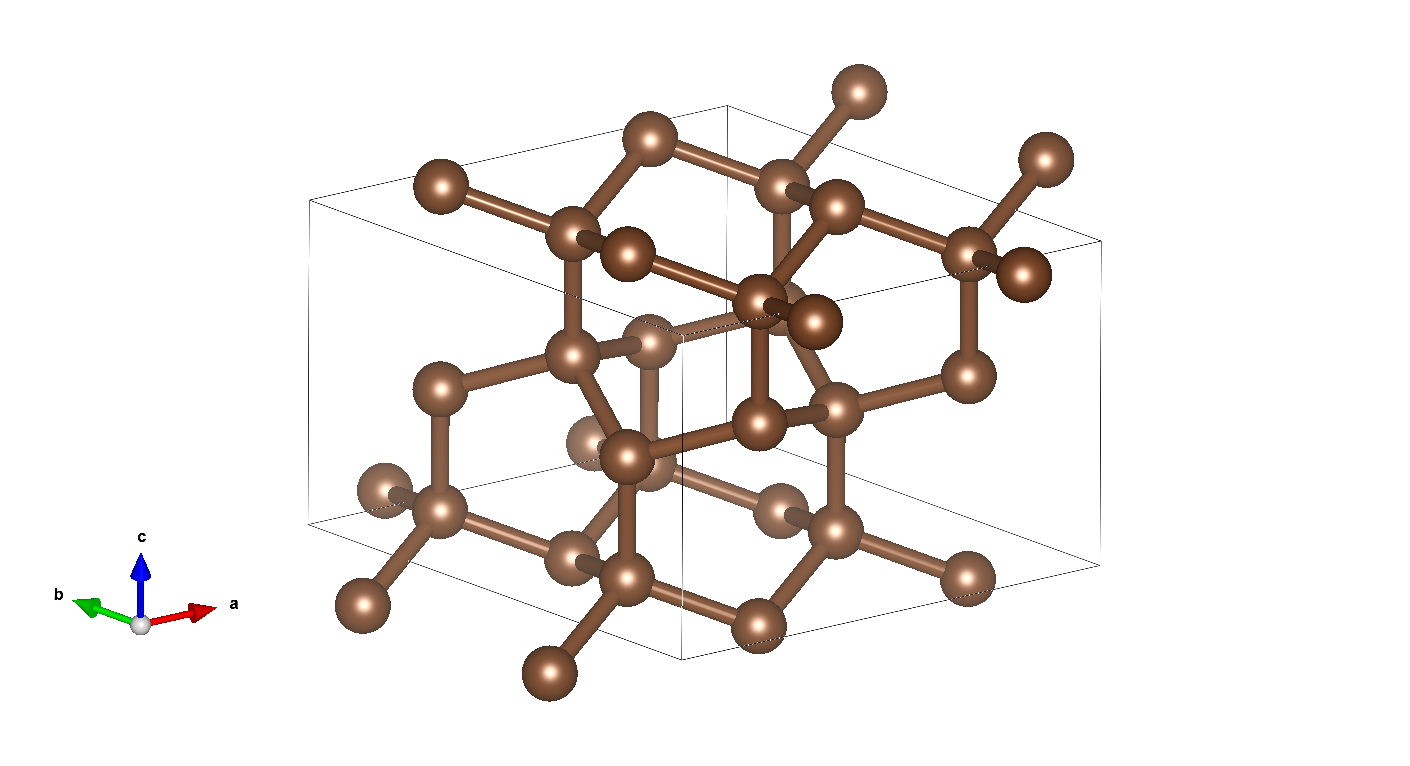
\includegraphics[width=0.5\textwidth, trim=0 0 27em 0,clip]{images/poscar_hex_16_birdseye.png}
  \end{center}
\end{frame}

\begin{frame}{Defected hexagonal diamond}
  \begin{center}
    \begin{tabular}{cr}
      Cubic diamond   & 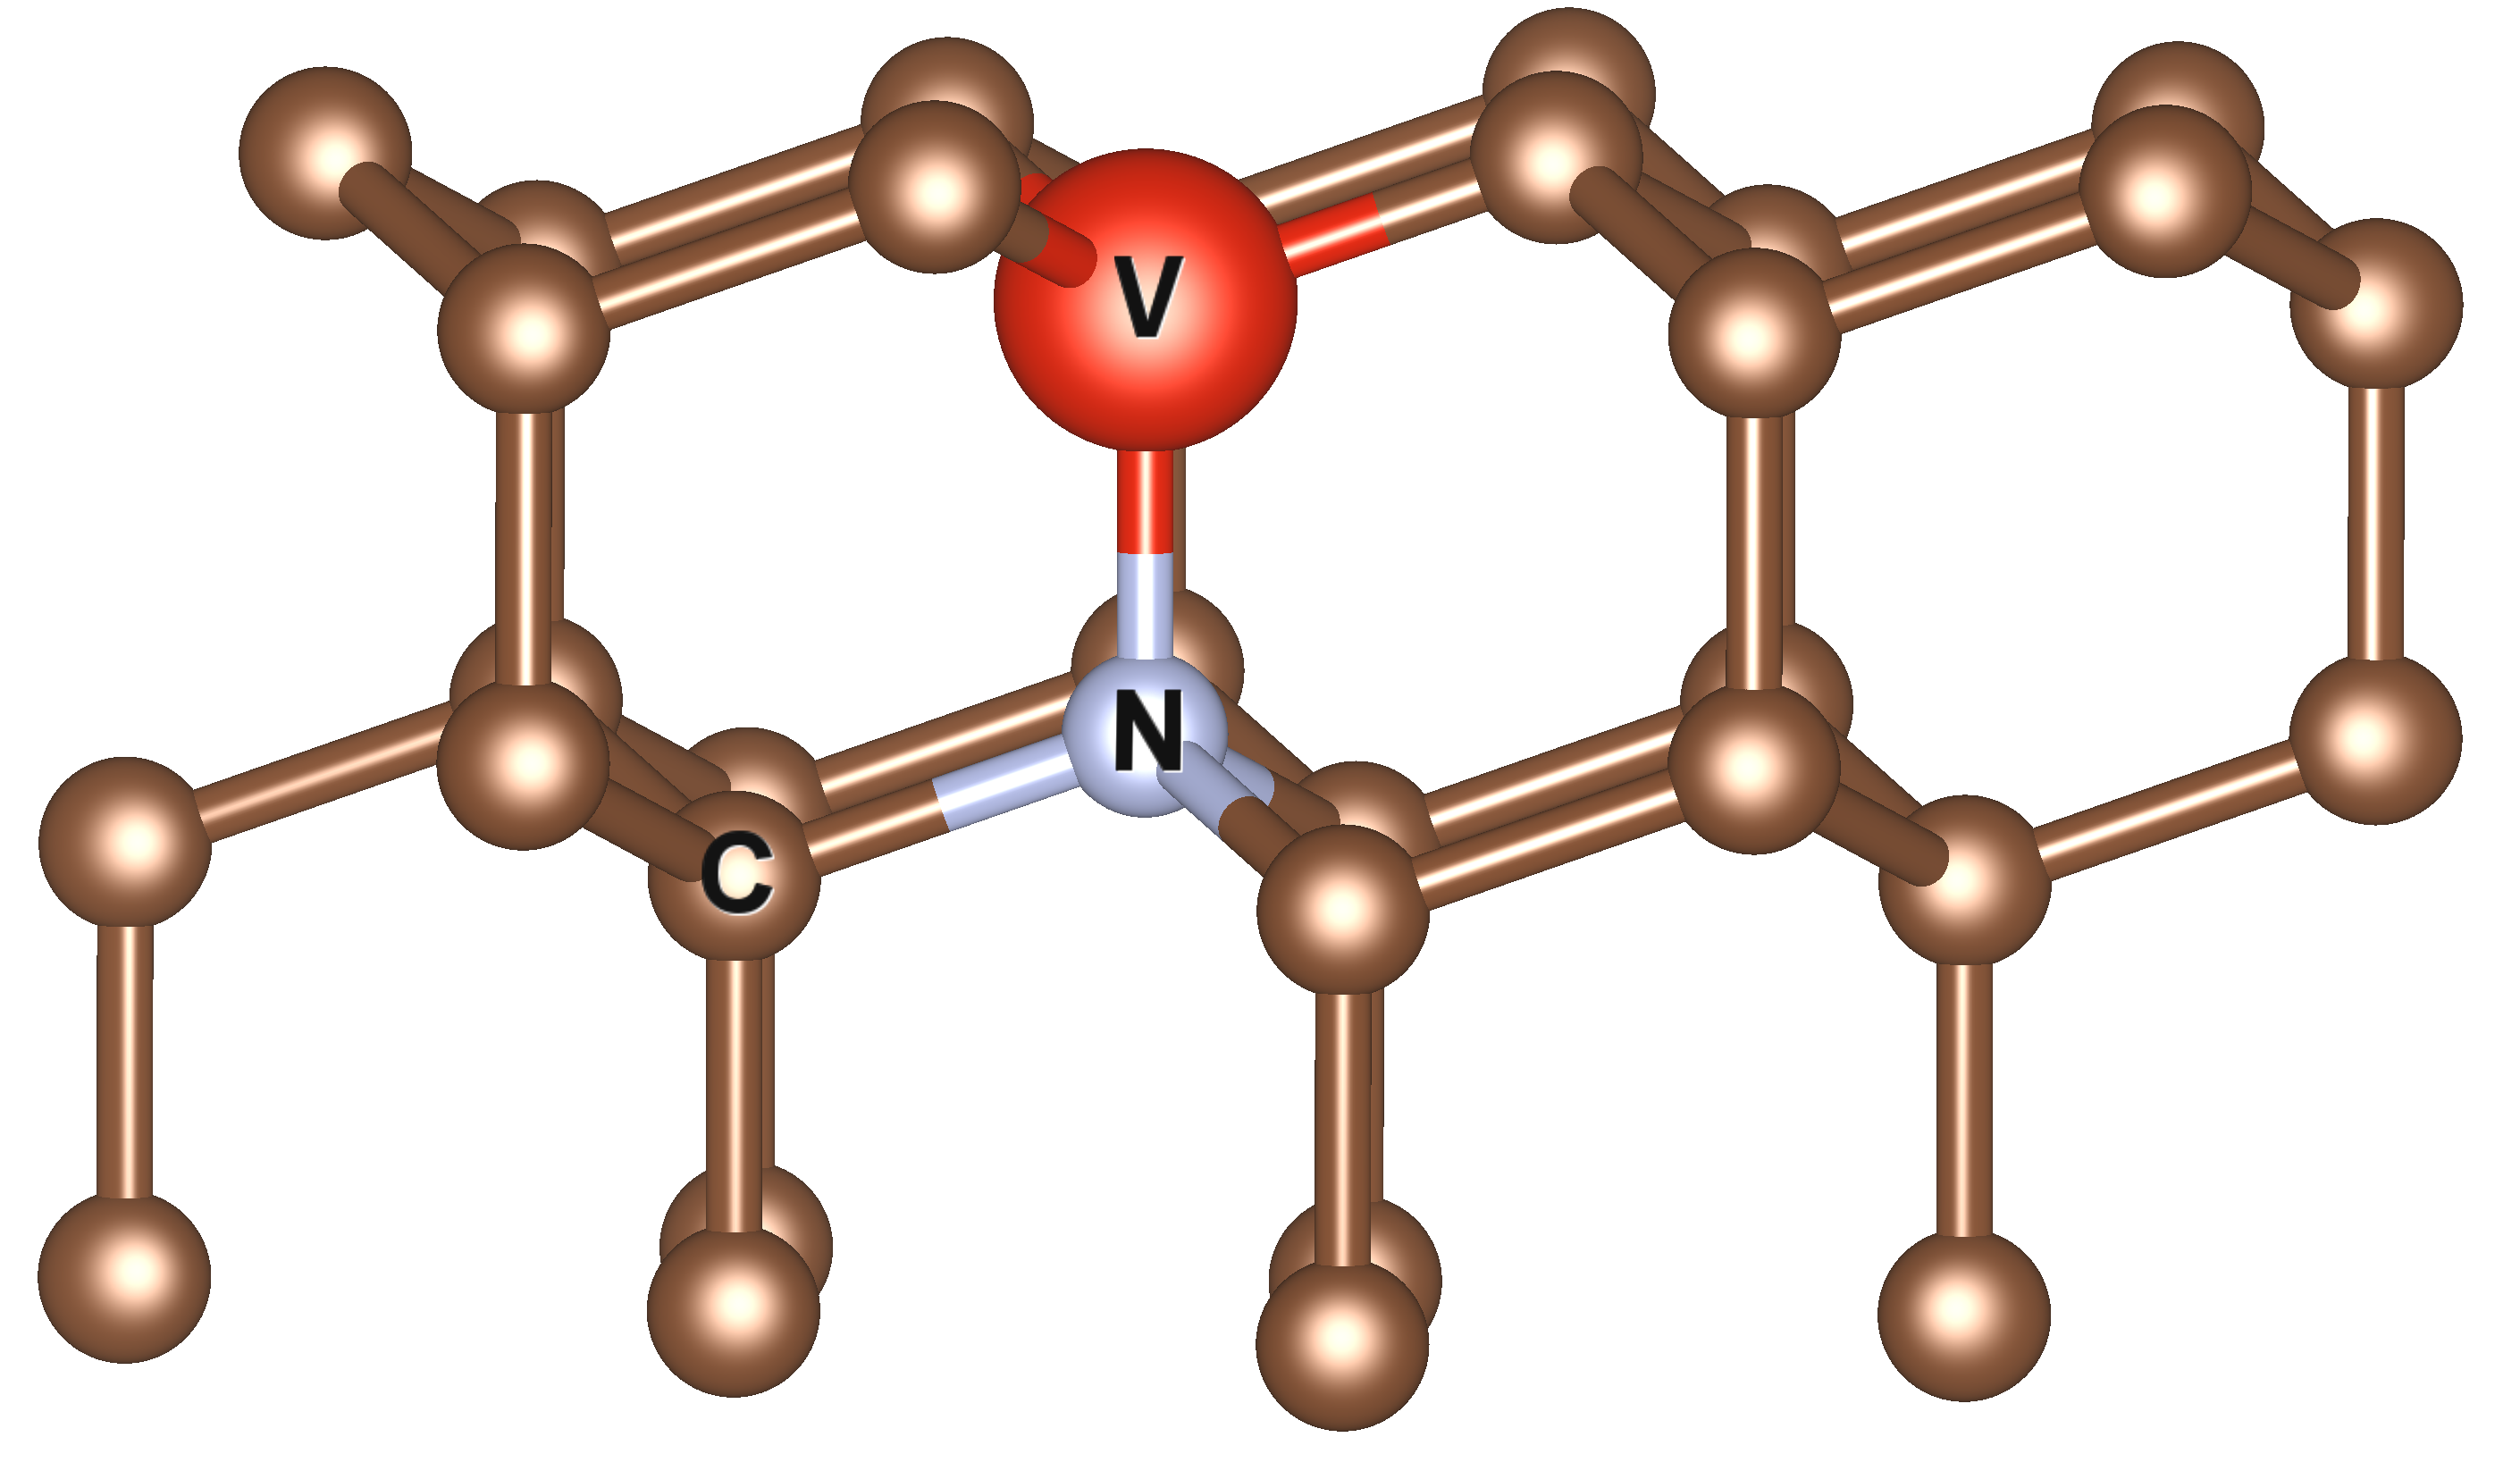
\includegraphics[width=0.4\textwidth]{images/POSCAR_16_view.png}\\
      Hexagonal $ x $-type &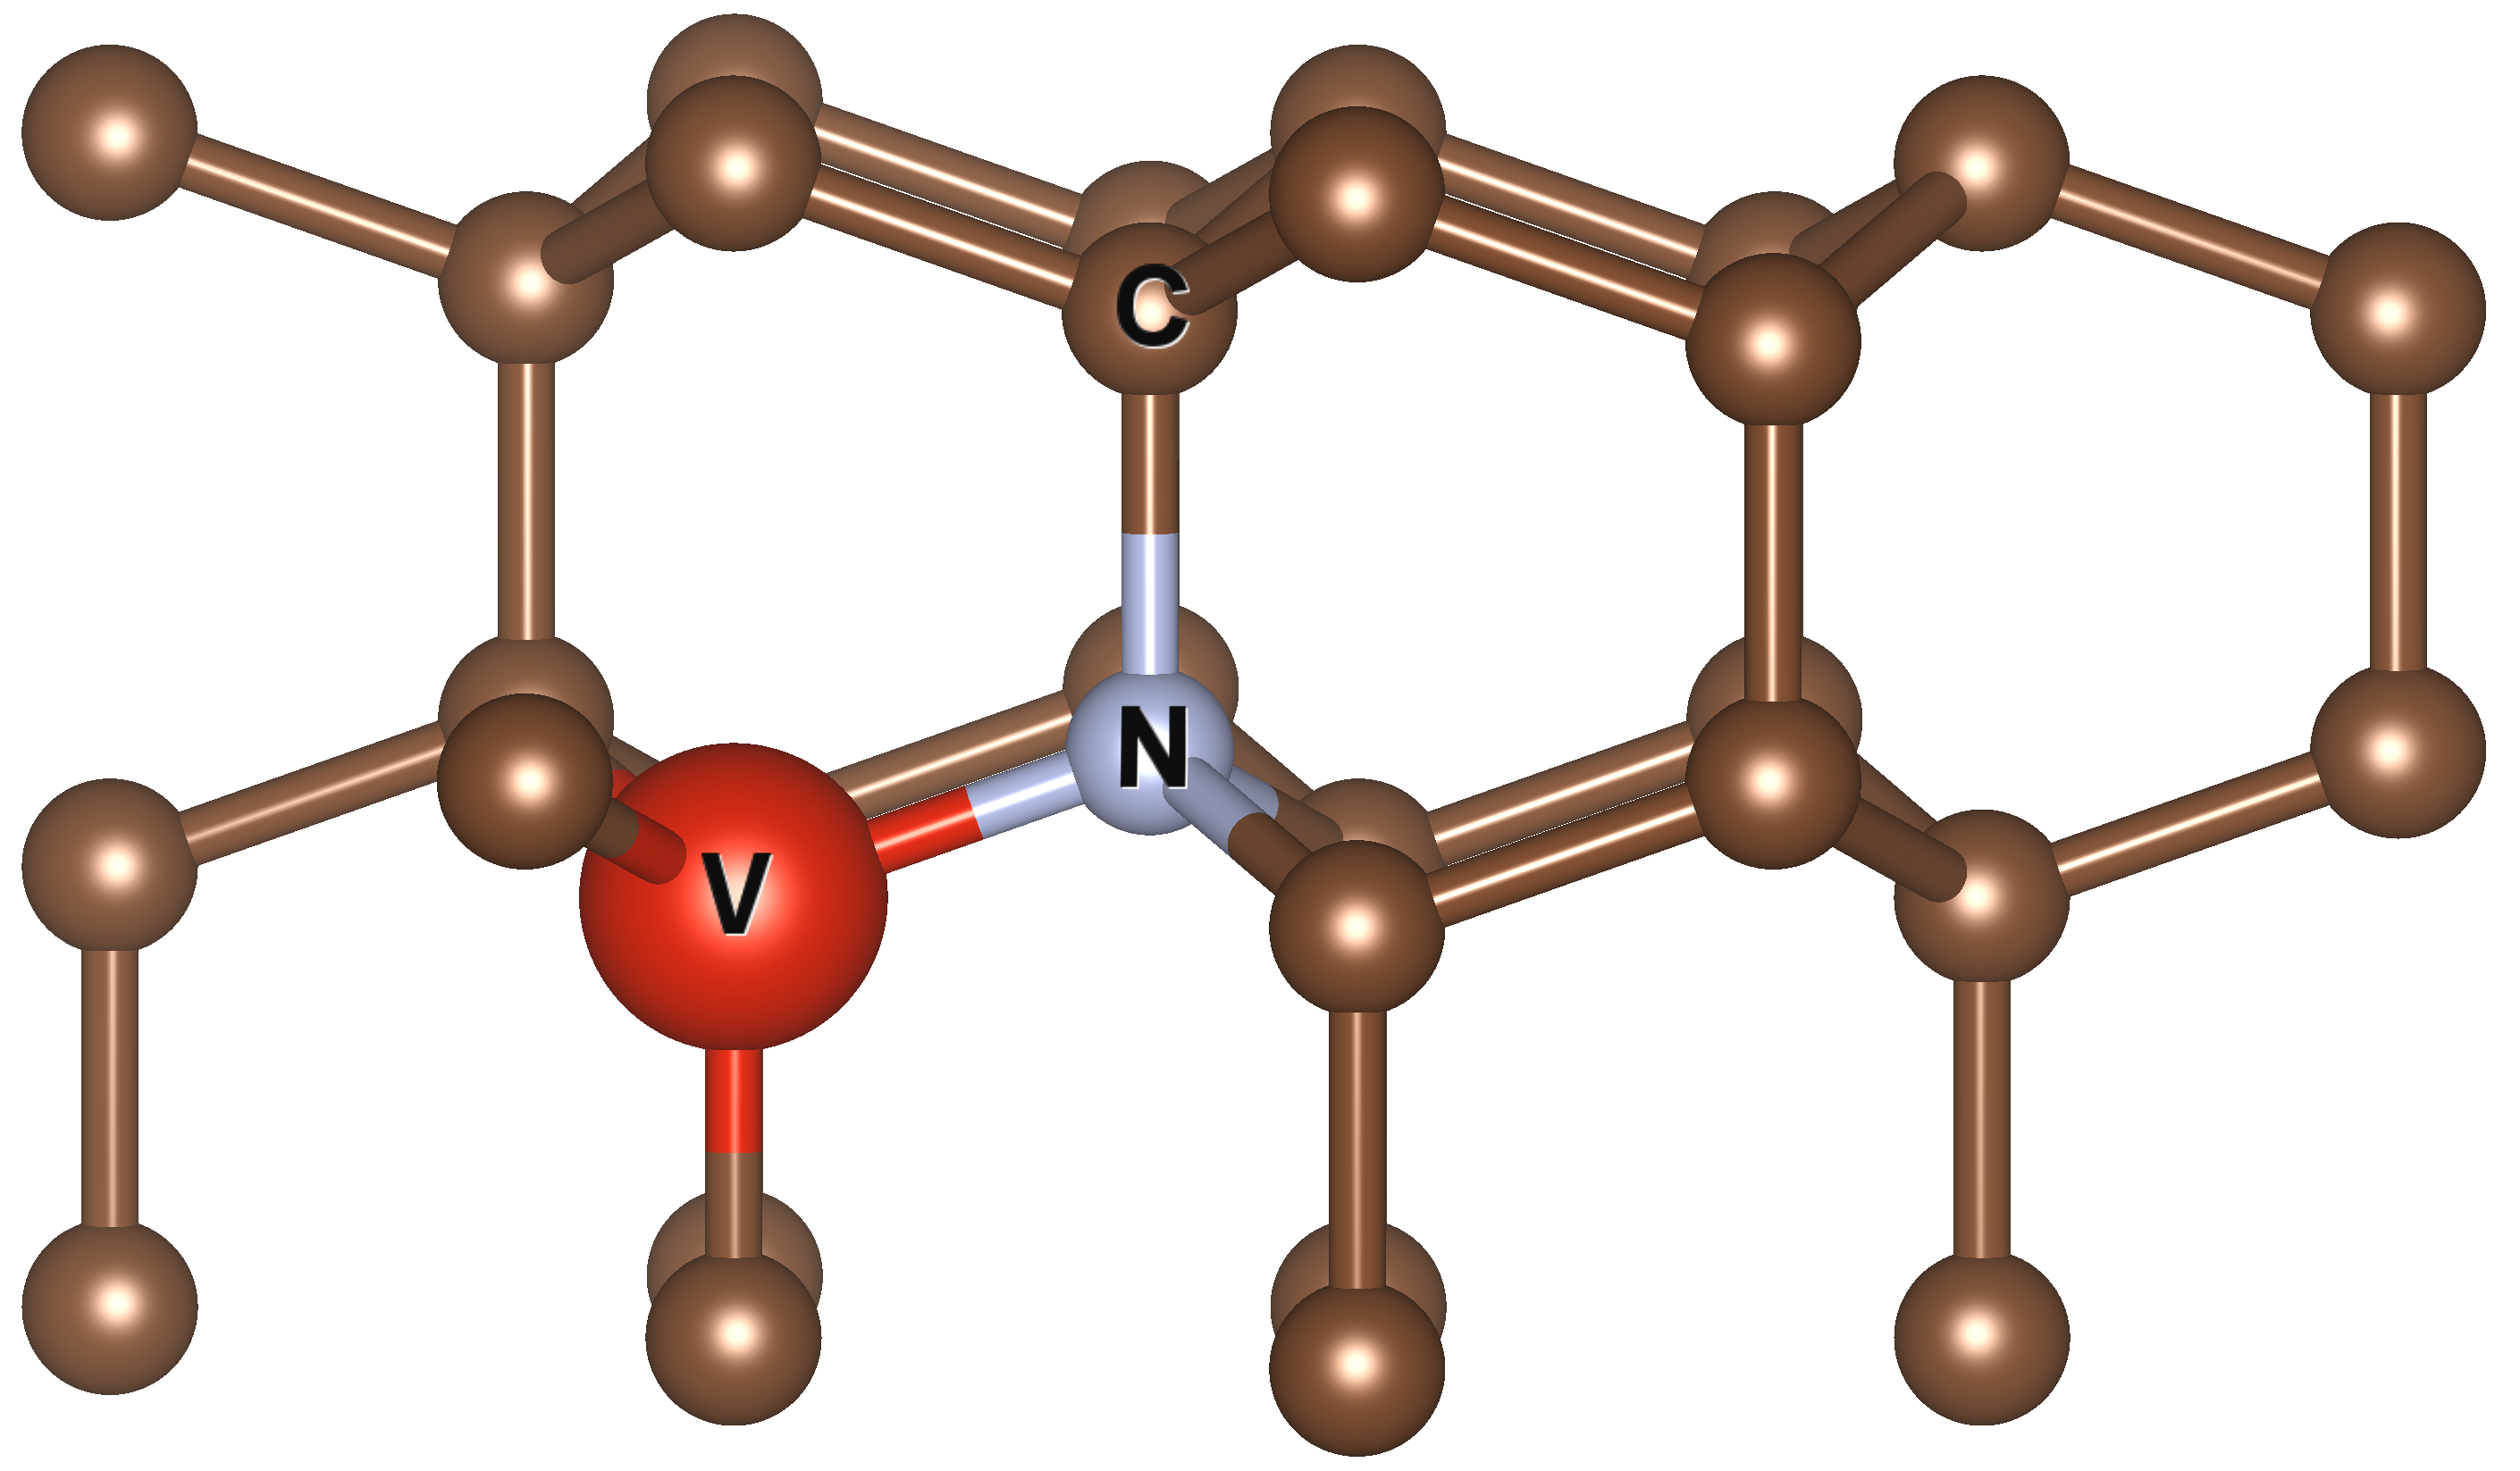
\includegraphics[width=0.4\textwidth]{images/POSCAR_16_x_view.png}\\
      Hexagonal $ z $-type & 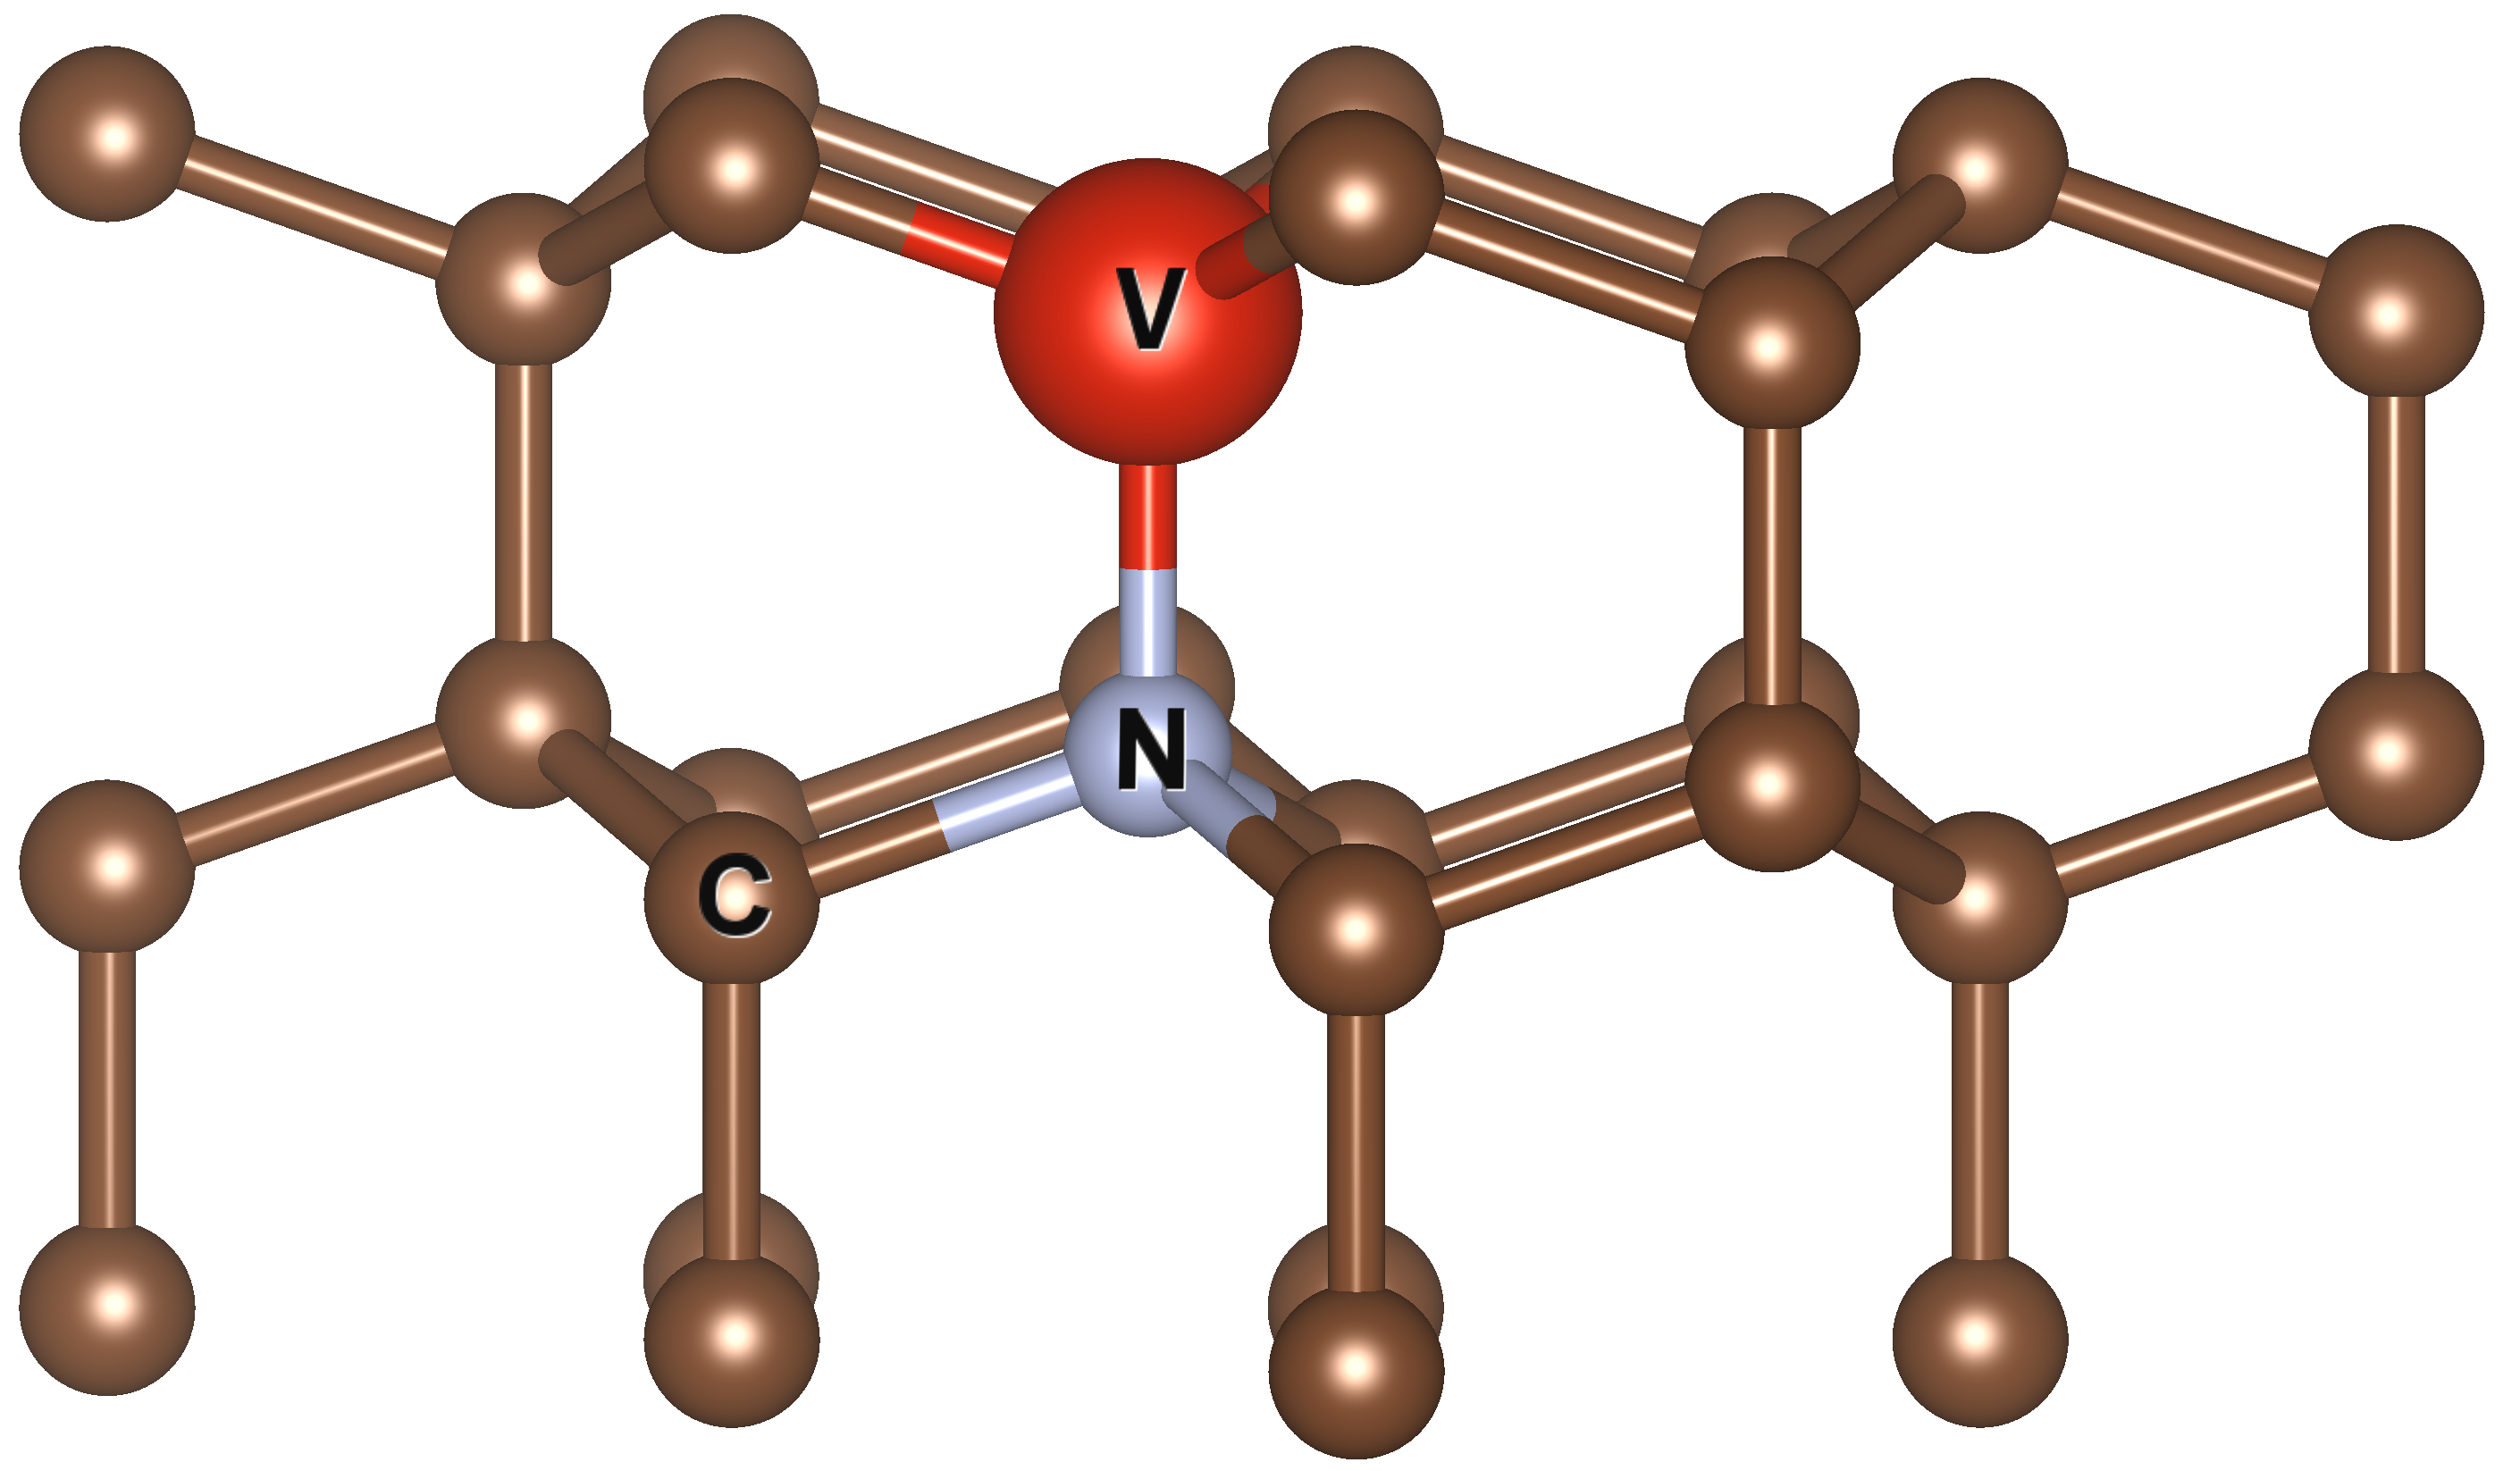
\includegraphics[width=0.4\textwidth]{images/POSCAR_16_z_view.png}
    \end{tabular}
  \end{center}

\end{frame}



\begin{frame}{Split vacancies: $ \mathsf{SiV}^{-} $  }
  \def\splitTrim{6}
  \def\splitTrimVertical{2}
  \begin{columns}
    \begin{column}{0.5\textwidth}
      \includegraphics[width=\textwidth, keepaspectratio,trim=\splitTrim cm \splitTrimVertical cm \splitTrim cm \splitTrimVertical cm,clip]{images/poscar__si_minux_definitiv_1.pdf}
    \end{column}
    \begin{column}{0.5\textwidth}
      \includegraphics[width=\textwidth, keepaspectratio,trim=\splitTrim cm \splitTrimVertical cm \splitTrim cm \splitTrimVertical cm,clip]{images/contcar__si_minux_definitiv_1_cartesian.pdf}
    \end{column}
  \end{columns}
\end{frame}

%\subsection*{XV-centers in cubic and hexagonal diamond}

\section{Results} %{{{1

\begin{frame}{$ \mathsf{NV}^{-} $: ZFS }
  \begin{itemize}
    \item 
      \textit{Cubic diamond, convergence and comparison with the experimental result.}
  \end{itemize}
  \includegraphics[width=1.0\textwidth, trim=0 0 0em 0,clip]{images/zfs_cubic/plot_cubic.pdf}
\end{frame}

\begin{frame}{$ \mathsf{NV}^{*} $: ZFS cubic ($ \mathsf{NV}^{*}_{c} $), Hexagonal $ x,z $ ($ \mathsf{NV}_{x,z}^{*} $)   }
  \includegraphics[width=1.0\textwidth, trim=0 0 0em 0,clip]{images/splitting_comparison/dmatrix_encut/N_all.pdf}
\end{frame}

\begin{frame}{ $ \mathsf{NV}^{-} $: Ground state}
  \begin{center}
    \begin{columns}
      \begin{column}{0.3\textwidth}
        \includegraphics[height=0.9\textheight, trim=0 0 0em 0,clip]{images/lumos/N_minus_cubic_128_dmatrix_encut_lumos.pdf}
      \end{column}
      \begin{column}{0.3\textwidth}
        \includegraphics[height=0.9\textheight, trim=0 0 0em 0,clip]{images/lumos/N_minus_hexagonal_z_128_dmatrix_encut_lumos.pdf}
      \end{column}
      \begin{column}{0.3\textwidth}
        \includegraphics[height=0.9\textheight, trim=0 0 0em 0,clip]{images/lumos/N_minus_hexagonal_x_128_dmatrix_encut_lumos.pdf}
      \end{column}
    \end{columns}
  \end{center}
\end{frame}


\begin{frame}{Expanding the defect}
  \begin{center}
    \includegraphics[width=0.5\textwidth]{images/elements.pdf}
  \end{center}
\end{frame}






\section{Summary} %{{{1




\begin{frame}{Where we are, and where to go next\ldots}
  \begin{itemize}
    \item Structural properties
    \item ZPL calculation.
    \item ZFS tensor calculation.
    \item \textbf{Beyond the Ground state:}\\
      Using DMRG for excited state calculations
  \end{itemize}
\end{frame}




\plain{Thank you!}





\end{document}



\end{document}


% vim: spell fdm=marker :
%vim-run: pdflatex %; make all
%vim-run: make all
